\documentclass[11pt, a4paper, DIV=12]{scrartcl}

% useful packages 
\usepackage{mathtools}
\usepackage{physics}
\usepackage{graphicx}					  
\graphicspath{{figs/}}



\usepackage{amssymb}
\usepackage{amsmath}
\usepackage{hyperref}
\usepackage[separate-uncertainty=true]{siunitx}
\usepackage{xcolor}
\usepackage{braket} % easy braket notation
\usepackage{enumitem}
\usepackage{booktabs}
\usepackage{here}
\usepackage{cprotect}

\usepackage[backend=biber, sorting=none]{biblatex}
\bibliography{refs.bib}

% \numberwithin{equation}{section}

\title{Error analysis of a Markov Chain}
\date{\today}
\author{Harilal Bhattarai \& Marcel Schindler}
\begin{document}
	\maketitle
	
\section{Introduction}
In this week’s exercise we apply proper analysis techniques to estimate the statistical error of a quantity estimated from a Markov Chain (MC). To do this exercise we can use most of the needed expression from previous exercise-sheets. In theory part, we only introduce some expressions and  we will try to illustrate the question with our findings and logic in the analysis part.
\section{Theory}
	The Markov Chain has reached the equilibrium distribution we use the usual ensemble mean
	\begin{equation}
	\bar{m}_{N}= \frac{1}{N}\sum_{k=1}^{N} m(\phi_{k})
	\end{equation}
	as the Monte-Carlo estimator of the magnetization $ <m> $.\\
	
	\textbf{Autocorrelation}
	A useful quantity in which to analyze the correlations is the autocorrelation function,
	\begin{equation}
	C(\tau)= \frac{\bar{\Gamma}^{m}(\tau)}{\bar{\Gamma}^{m}(0)}
	\end{equation}
	Where; 
	$  
	\Gamma^{(m)}(|k -l|)= <(m(\phi_{k}) - <m>) <(m(\phi_{l}) - <m>) $
	
	\textbf{Blocking}: It is also called binning.\\
	\textbf{The bootstrap}
	
\section{Analysis}
To compare the two MC trajectories, we set $\beta \text{J}= 0.1 $; $\beta \text{h}= 0.5 $; n=5; for two different number of integration steps $ N_{md}=4$ and  $\text{N}_{md}= 100 $. we generate long MC for each run $ \text{N}=12800 $. To simulating this Markov Chain we took sampling HS field configurations $ \phi_{1}, \phi_{2}, \dots \phi_{N} $ for given number N of trajectories with the HMC. From this simulation and graphing we have output figure \ref{fig:comperision_4_100} for the magnitization. From our research we got success rate for $ N_{md}=4$ is 6207 and $ N_{md}=100 $ is 12800. We only look at the last 8000 points, so we do not have to deal with thermalization. So we get way more Points for $N_{md}$ equals 100 and also the points are more divers.
	
\begin{figure}[H]
		\centering
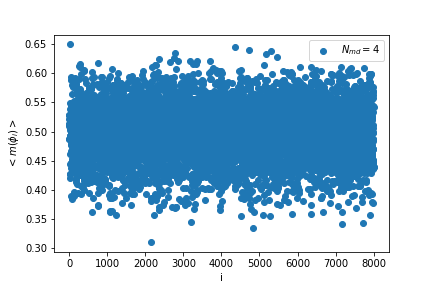
\includegraphics[width=0.6\linewidth]{comparison_magnitization_4.png}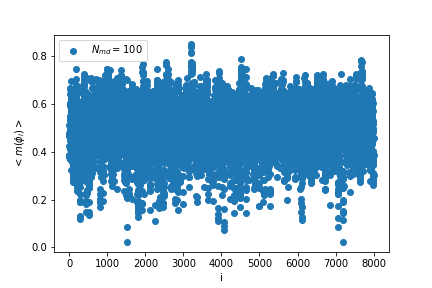
\includegraphics[width=0.6\linewidth]{comparison_magnitization_100.png}
\caption{Trajectories of the MC history of magnetization with different number of integration steps. Here, two graphs are at $ N_{md}=4$ and $ N_{md}=100$.}
	\label{fig:comperision_4_100}
\end{figure}

	
\textbf{Autocorrelation}: An autocorrelation plot is one of the best way to check the randomness present in data. To determine the autocorrelation of time-series in dataset we plotted a functional decay nature of autocorrelation estimator function. From output graph \ref{fig:autocorrelation} we notice that in the first some lags it try to follow the exponentially decreasing path; however, when it reached very close to zero correlation estimator value then at the higher time lags there is the absence of any significance pattern. The data sets are fluctuate below and above the zero point. Therefore, it shows the quite randomness of the data set with time-series.
	
	\begin{figure}[H]
		\centering
		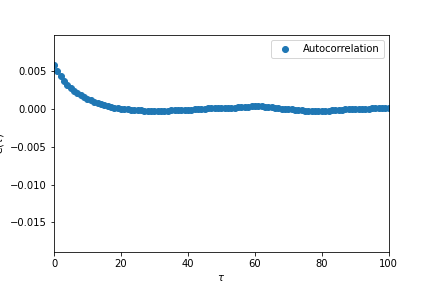
\includegraphics[width=0.6\linewidth]{autokorrelation.png}
		\caption{Plot of the function of straightforward estimator $ C(\tau) $ to generated data sets.}
		\label{fig:autocorrelation}
	\end{figure}
	
\textbf{Blocking}: It is also called binning. It is used to reduce the variance.
To do so, we used the data generated for b= 2, 4, 8, 16, 32 and 64 with $ \text{N}_{\text{md}}=100 $ and calculated the autocorrelation for each block list. Afterward, we plotted the decay of autocorrelation function C$ (\tau) $ with time $ \tau $ and standard deviation of the blocked list, \ref{fig:blockingAutocorrelation} are the output graphs.
	
From fig \ref{fig:blockingAutocorrelation} we can see that the the autocorrelation function decay exponentially and follow the linear path.The autocorrelation function is plotted for two values of  in Figure 8.8. Furthermore, we notice that for small value of \text{b}(for b=2, 4, 8) the autocorrelation corresponds to the expected outcome. With higher b the autocorrelation decreases faster. This we also expect since the blocks correlate less to eachother. For higher b we get a strange graph. This is maybe because if we take so big block sizes we do not have much data. We would expect for higher b that it would decrease faster then lower b and stays at zero. We get actully randomize points with negativ values.
	
	\begin{figure}[H]
		\centering
		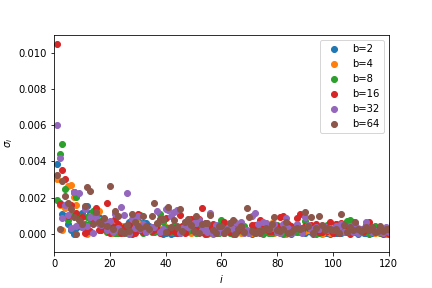
\includegraphics[width=0.6\linewidth]{blocking_standard_deviation.png}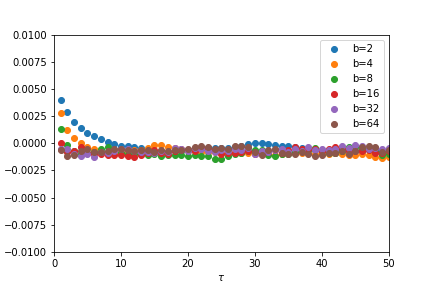
\includegraphics[width=0.6\linewidth]{blocking_autokorrelation.png}
		\caption{ The autocorrelation for blocked data for b= 2, 4, 8, 16, 32, and 64. Left figure describe the decay of autocorrelation function $ C(\tau) $ and right graph for standard deviation of blocked list.}
		\label{fig:blockingAutocorrelation}
	\end{figure}
	
\textbf{The bootstrap}: In this section, we have to calculate the stability of the error as a function of $ \text{N}_{\text{bs}} $. To do so, we used the procedure to the bootstrap as given in the exercise-sheet. The bootstrap method converges on the value $\approx 0.0003$(without skaling). We can see that the errors are actully quite in the same region but the standard error varries a lot. So it is not easy to make a good estimate of the error. Often we overestimate the error with the standard error.
	
	\begin{figure}[H]
		\centering
		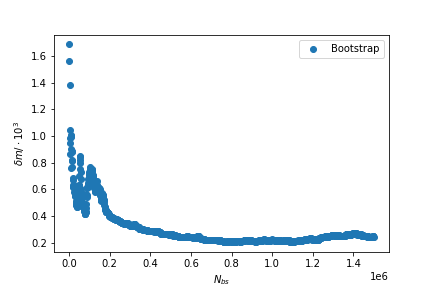
\includegraphics[width=0.6\linewidth]{bootstrap.png}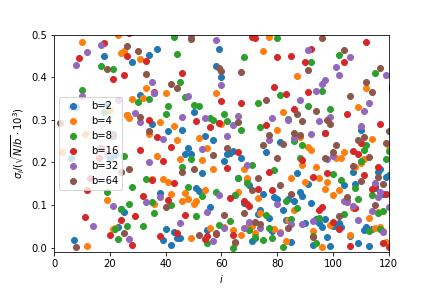
\includegraphics[width=0.6\linewidth]{blocking_standard_deviation_test.png}
		\caption{ The stability of the bootstrap error as a function of $ N_{bs} $(left) and the standard error(right).}
		\label{fig:boottrap}
	\end{figure}

\section{Conclusion}
From our research, we conclude that, the success rate for higher $ N_{md} $ is more. We have found for $ N_{md}=4$ is 6207 and $ N_{md}=100 $ is 12800. So it is an advantage to take higher $N_{md}$. We also saw that the standard error is not a good parameter to calculate the error. it is nearly in the same region but varies a lot. So the bootstrap method has way more advantages. The presicion is higher and it converge to a value.
	
\begin{thebibliography}{12}
\bibitem{exercise-sheet} 
Thomas Luu, Andreas Nogga, Marcus Petschlies and  Andreas Wirzba, Exercise-sheet, 2020. 
\end{thebibliography}	
\end{document}